\section{Introduction}\label{introduction}

Multimodal sentiment analysis (MSA) predicts affective polarity or
intensity from language, acoustic behavior, and visual behavior. The
task was established through in-the-wild opinion-video analysis and
later scaled through CMU-MOSEI
\cite{zadeh2016multimodal, zadeh2018mosei}. Text often carries the
dominant semantic signal, whereas voice and face provide complementary
evidence about emphasis, timing, and non-verbal expression. This
complementarity is valuable only when the contributing modalities are
trustworthy. Background noise, occlusion, temporal misalignment, missing
segments, and preprocessing artifacts can make the usefulness of a
modality vary across samples even when the dataset provides all three
streams.

Quality-aware methods address this variability by estimating modality
quality and using the resulting score to control fusion, attention,
expert routing, or optimization. Dynamic fusion has been formulated
through uncertainty-aware weighting and generalization analysis
\cite{zhang2023qmf}, predictive confidence calibration
\cite{cao2024pdf}, and continuous reliability-aware expert routing
\cite{zhu2026qamoe}. Other approaches supervise attention with original
and corrupted features \cite{mai2025samlml}, construct proxy modalities
for incomplete inputs \cite{zhu2025prmf}, coordinate weak modalities
through sample-level trust \cite{he2026ebmc}, or calibrate
representations and gradients \cite{jiang2026cpsc}. These methods
differ substantially, but they share a latent premise: the intermediate
score called \emph{quality}, \emph{confidence}, \emph{trust}, or
\emph{reliability} represents the property that the downstream mechanism
assumes it represents.

Producing a score, however, does not establish this premise. A score can
vary because sequence length or feature energy varies; it can be reduced
across the batch and therefore cease to be sample-specific; or it can
enter a computational graph whose downstream prediction is effectively
insensitive to it. Robustness analysis has already shown that clean-set
accuracy is insufficient for characterizing MSA under modality
perturbations \cite{hazarika2022robustness}. More directly,
leakage-safe score permutation can reveal that an apparently
quality-aware fusion model barely depends on its quality scores
\cite{moon2026quality}. These observations motivate a stricter question
than whether a quality-aware model attains a favorable test score:
\textbf{is the quality signal itself measurable, non-confounded, and
causally connected to the claimed optimization mechanism?}

We encountered this question while extending MFON, a prompt-based
architecture that improves acoustic and visual representations through
frozen unimodal teachers, knowledge distillation, and cross-modal
contrastive learning \cite{zhang2025mfon}. An initial prototype added
adaptive auxiliary weights, dynamic prompts, and norm-based curriculum
selection. Three-seed evaluation did not show stable improvement over a
repaired MFON baseline. Implementation and data audits then identified
structural reasons not visible from the final metrics: sample scores had
been averaged into batch scalars; distillation and contrastive losses
had already been reduced before weighting; unconstrained non-negative
auxiliary coefficients had a direct gradient incentive to shrink; and
the norm-based curriculum score was dominated by effective sequence
length and increased when noise was added.

These failures changed the aim of the work. Instead of proposing another
fusion module, we treat modality reliability as an auditable
intermediate variable and ask how it can control training without
changing the total amount of auxiliary supervision. The resulting
pipeline has two components. First, lightweight visual and acoustic
heads learn an ordered reliability relation from clean, mildly
corrupted, and strongly corrupted features. Second, reliability
redistributes per-sample KL and InfoNCE losses within each mini-batch
while an exact finite-batch constraint preserves the original mean
auxiliary weights. An allocation warmup interpolates from uniform to
reliability-aware assignment without scaling down the total budget. This
distinction is crucial: an improvement can otherwise arise simply
because the training objective received less auxiliary supervision
during early epochs.

The current study makes four evidence-bounded contributions:

\begin{enumerate}
\def\labelenumi{\arabic{enumi}.}
\tightlist
\item
  We formulate a five-part audit for modality quality signals, covering
  sample granularity, monotonic response to controlled degradation,
  sensitivity to non-quality confounds, actionability, and collapse of
  dynamic weights.
\item
  We provide a reproducible failure analysis of an MFON-based prototype,
  including a norm proxy that correlates with effective sequence length
  and assigns higher scores to more strongly corrupted features.
\item
  We implement interventional reliability learning and exact
  finite-batch redistribution of per-sample distillation and contrastive
  losses. The final P4 schedule (an implementation label retained for
  traceability) keeps the mean auxiliary budget
  identical to the repaired MFON baseline from the first epoch.
\item
  We report an exploratory three-seed CMU-MOSI study and a frozen-protocol
  three-seed CMU-MOSEI replication, then use Gaussian, held-out corruption,
  and cross-sample target-fidelity audits to separate degradation detection
  from the properties required by allocation. The validation audit falsifies
  cross-sample KL fidelity for vision and finds only weak acoustic support.
\end{enumerate}

\section{Related Work}\label{related-work}

\subsection{Multimodal sentiment analysis and weak-modality
optimization}\label{multimodal-sentiment-analysis-and-weak-modality-optimization}

Early MSA architectures explicitly modeled cross-modal interactions
through tensor fusion \cite{zadeh2017tensor}, recurrent memory over
multiple views \cite{zadeh2018memory}, and low-rank factorization of
modality-specific interactions \cite{liu2018efficient}. This line
established that complementary cues can be modeled beyond direct
concatenation, but it assumed relatively stable aligned inputs and did
not make reliability an independently audited variable.

Representation learning subsequently shifted toward cross-modal
attention and more explicit separation of shared and modality-specific
information. MulT uses directional cross-modal attention for unaligned
language sequences \cite{tsai2019multimodal}, MAG injects multimodal
information into a pretrained language transformer
\cite{rahman2020integrating}, and MISA separates modality-invariant and
modality-specific representations \cite{hazarika2020misa}.
Self-supervised modality-specific objectives \cite{yu2021learning} and
hierarchical mutual-information maximization \cite{han2021improving}
further strengthen individual and shared representations. These methods
improve how modalities are encoded, but their representation objectives
do not by themselves verify whether a sample-wise quality score measures
degradation.

Recent models explore unified task learning \cite{hu2022unimse},
MLP-based interaction \cite{sun2022cubemlp}, language-guided
hyper-modality representations \cite{zhang2023learning}, text-enhanced
transformer fusion \cite{wang2023tetfn}, and multi-loss fusion
\cite{wu2024multimodal}. MFON targets under-optimized acoustic and
visual streams through modality prompts, unimodal-teacher distillation,
and cross-modal contrastive objectives \cite{zhang2025mfon}.
Sample-level modality valuation shows that modality contribution cannot
be summarized adequately by a dataset-level average \cite{wei2024smv},
while EBMC combines weak-modality enhancement, energy-guided
coordination, and sample-level trust \cite{he2026ebmc}. These studies
motivate per-sample treatment, but per-sample weighting alone is
insufficient: the weighting signal and the amount of supervision it
controls must both be verified.

\subsection{Example reweighting and curriculum
learning}\label{example-reweighting-and-curriculum-learning}

Sample allocation has a broader history than quality-aware MSA. Self-paced
learning prioritizes easier examples and gradually expands the training set
\cite{kumar2010selfpaced}, whereas validation-driven meta-reweighting chooses
example weights through their gradient effect on a clean validation objective
\cite{ren2018reweight}. In MSA, curriculum learning has also been used to order
weakly supervised cross-modal pairs by estimated difficulty, while discarding
the hardest pairs as potential noise \cite{mai2022curriculum}. These methods
make clear that emphasizing reliable or easy samples is not the only plausible
direction: hard-example and validation-utility rules encode different
objectives. Our fixed-budget construction controls total auxiliary supervision,
but the direction and score--sample correspondence remain empirical hypotheses
that require inverse and permuted controls.

\subsection{Quality-aware learning under degraded or incomplete
modalities}\label{quality-aware-learning-under-degraded-or-incomplete-modalities}

Robust MSA has been approached through feature reconstruction,
decision-level uncertainty, confidence calibration, supervised
corruption, proxy reconstruction, and expert routing. TFR-Net
reconstructs modality features to improve prediction under imperfect
inputs \cite{yuan2021transformer}. QMF derives dynamic fusion from
modality quality and studies its generalization behavior
\cite{zhang2023qmf}, whereas predictive dynamic fusion distinguishes
local and holistic confidence and applies relative calibration
\cite{cao2024pdf}. SAM-LML uses original, corrupted, and noise-only
features to supervise attention ordering \cite{mai2025samlml}. P-RMF
handles incomplete inputs through probabilistic proxy modalities
\cite{zhu2025prmf}, and QA-MoE models a continuous reliability spectrum
for expert routing \cite{zhu2026qamoe}. CPSC calibrates both
representations and gradients through conformal prediction
\cite{jiang2026cpsc}. DEAR estimates reconstruction fidelity under missing
modalities and uses it to gate synergistic and robust inference streams
\cite{zou2026dear}. QMF, QA-MoE, and DEAR use quality or reliability to
alter prediction-time fusion or routing, whereas P4 confines
reliability to training-time auxiliary allocation and leaves the
inference fusion graph unchanged. Our method does not claim that
corruption-based ranking or quality-aware weighting is itself new. Its narrower
distinction is to audit the score as an intermediate variable and
compare allocations under an exactly matched training-time auxiliary
budget.

\begin{table*}[t]
\caption{Mechanism boundary relative to representative quality-aware and
sample-allocation methods. ``Ordinal'' refers to within-sample ordering under
controlled corruption; it does not imply cross-sample calibration.}
\label{tab:related-boundary}
\centering
\small
\setlength{\tabcolsep}{4pt}
\begin{tabularx}{\textwidth}{lYYY}
\toprule
Method & Signal & Stage and control & Main boundary \\
\midrule
Meta-reweighting \cite{ren2018reweight} & Validation gradient & Training; example loss & Validation utility \\
MSA curriculum \cite{mai2022curriculum} & Pair difficulty & Training; pair schedule & Easy-to-hard order \\
QMF \cite{zhang2023qmf} & Uncertainty/quality & Inference; modality fusion & Prediction robustness \\
SAM-LML \cite{mai2025samlml} & Ordered corruption & Training; representation & Low-quality learning \\
QA-MoE \cite{zhu2026qamoe} & Reliability spectrum & Inference; expert routing & Continuous routing \\
DEAR \cite{zou2026dear} & Reconstruction error & Inference; dual-stream gate & Missing modalities \\
This study & Ordinal response & Training; auxiliary losses & Exact batch budget and score audit \\
\bottomrule
\end{tabularx}
\end{table*}

\subsection{Diagnosing quality
signals}\label{diagnosing-quality-signals}

Most robustness studies evaluate predictions after perturbing one or
more modalities \cite{hazarika2022robustness}. This is necessary but
does not establish what an internal quality score measures. A useful
score must remain sample-specific, decrease under controlled
degradation, avoid trivial dependence on sequence length or energy, and
change the mechanism it purportedly controls. Score permutation offers
one actionability test by holding the model and inputs fixed while
breaking the score--sample correspondence \cite{moon2026quality}. We
extend this diagnostic perspective to both representation and
optimization: the audit examines tensor granularity, degradation
ranking, confounds, prediction or gradient dependence, and whether
learned auxiliary weights can reduce the objective by collapsing
globally.

\section{Problem Formulation}\label{problem-formulation}

Consider a batch of \(B\) samples. Sample \(i\) contains text, visual,
and acoustic features

\[
x_i=\{x_i^t,x_i^v,x_i^a\}, \qquad y_i\in\mathbb{R},
\]

and the base model predicts sentiment intensity

\[
\hat y_i=F(x_i^t,x_i^v,x_i^a).
\]

MFON additionally produces trainable visual and acoustic embeddings
\(z_i^v,z_i^a\), frozen unimodal-teacher embeddings
\(\bar z_i^v,\bar z_i^a\), and a text embedding \(z_i^t\). Its auxiliary
objectives contain modality-specific KL terms and text--modality InfoNCE
terms. We denote their unreduced values by

\[
\ell^{\mathrm{KL}}_{v,i},\quad
\ell^{\mathrm{KL}}_{a,i},\quad
\ell^{\mathrm{NCE}}_{tv,i},\quad
\ell^{\mathrm{NCE}}_{ta,i}.
\]

For each non-text modality \(m\in\{v,a\}\), a reliability head produces
\(q_i^m\in[0,1]\). We use \emph{input reliability} to mean whether a
feature sequence preserves its structure under the degradation process
modeled during training. This differs from \emph{task utility}: a clean
but emotionally neutral face may be reliable yet uninformative, while
mildly noisy speech may still carry a strong sentiment cue. The present
method estimates reliability for allocating training-time auxiliary
supervision; it does not replace the main sentiment objective with a
direct estimate of modality utility.

The supervision used below is ordinal within each original sample. It
establishes whether the score decreases along that sample's synthetic
degradation path; it does not, by itself, calibrate the absolute scores of two
different clean samples. Because allocation normalizes clean scores across a
mini-batch, cross-sample comparability and auxiliary-target fidelity are
additional assumptions rather than consequences of the ranking objective.

\section{Auditing Modality Quality
Signals}\label{auditing-modality-quality-signals}

\subsection{Sample granularity}\label{sample-granularity}

A sample-level score must be a vector
\(\mathbf q^m=[q_1^m,\ldots,q_B^m]\), not a scalar shared by the batch.
We audit the shape at the point where the score is consumed and test
whether a fixed sample retains its score when paired with different
companion samples. The same requirement applies to the controlled loss:
if an auxiliary loss has already been reduced across the batch,
multiplying it by a sample-wise vector cannot recover sample-wise
allocation.

\subsection{Degradation
monotonicity}\label{degradation-monotonicity}

Let \(C_m(x;s)\) denote a modality-specific corruption with severity
\(s\), where \(s=0\) is clean. A reliability score intended to measure
degradation should satisfy an ordered relation in expectation:

\[
s_1<s_2 \quad\Rightarrow\quad
\mathbb E[R_m(C_m(x;s_1))] > \mathbb E[R_m(C_m(x;s_2))].
\]

We quantify this relation with Spearman correlation between severity and
score, clean-versus-corrupt AUROC, and the fraction of highest-severity
samples whose score falls below the corresponding clean score.

\subsection{Confound sensitivity}\label{confound-sensitivity}

We measure the association between clean reliability scores and
effective sequence length, padding ratio, feature energy, sentiment
label, and absolute sentiment intensity. We also test transformations
that preserve valid content while changing padding or positive feature
scale. These checks do not prove that a head has learned a semantic
notion of quality, but they can falsify simple shortcuts that would make
the reliability interpretation untenable.

\subsection{Actionability}\label{actionability}

Actionability asks whether changing the score while holding other
factors constant changes predictions, gradients, or allocation-sensitive
performance. We compare learned scores with constant, permuted,
rank-reversed, and severity-derived controls when the corresponding
experiment uses the same average auxiliary budget. A score that passes
degradation detection but has no downstream effect remains a measurement
signal, not evidence for a useful allocation mechanism.

\subsection{Non-collapse}\label{non-collapse}

If non-negative auxiliary coefficients are learned freely in

\[
L=L_{\mathrm{task}}+\alpha_vL_v+\alpha_aL_a+\beta L_{\mathrm{NCE}},
\]

then \(\partial L/\partial\alpha_v=L_v\ge0\) creates a direct incentive
for gradient descent to reduce \(\alpha_v\). Declining weights therefore
cannot be interpreted automatically as learned task importance. A valid
comparison requires a normalization, budget, simplex, compensating
regularizer, or another mechanism that prevents the total auxiliary
supervision from shrinking unnoticed.

\section{Audited, Fixed-Budget Auxiliary
Learning}\label{audited-fixed-budget-auxiliary-learning}

\subsection{Overview}\label{overview}

The proposed training path preserves MFON's text encoder, modality
prompts, frozen unimodal teachers, KL distillation, InfoNCE alignment,
and sentiment decoder \cite{zhang2025mfon}. Our changes occur only in
the reliability and auxiliary-loss paths. For each visual and acoustic
input, the method constructs ordered corruptions, trains a
modality-specific reliability head, retains the four auxiliary losses at
sample resolution, and uses reliability to redistribute their weights.
The final P4 setting keeps the sentiment-task input clean and uses
synthetic corruptions only for reliability supervision. Thus, the main
comparison isolates training-time allocation from both inference-time
gating and corruption of the sentiment path.

Throughout the paper, ``reliability'' is shorthand for response under the
modeled Gaussian feature corruption. Where evidence concerns unseen
corruptions or cross-sample allocation, we use the narrower term
\emph{degradation-response score} to avoid implying general perceptual quality.

\begin{figure*}[t]
\centering
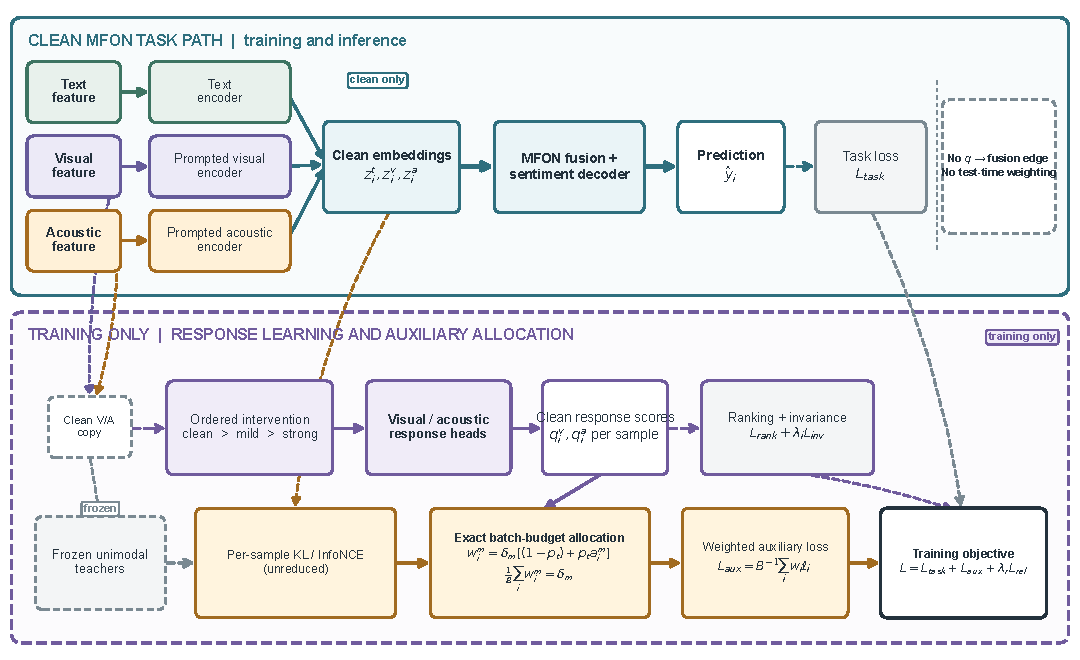
\includegraphics[width=\textwidth]{../figures/f1_method_overview_en.pdf}
\caption{Audited fixed-budget auxiliary learning with a clean inference
path. Clean text, visual, and acoustic features follow the unchanged MFON
task path to the sentiment decoder. During training only, ordered
clean--mild--strong interventions supervise visual and acoustic reliability
heads. Clean, sample-wise scores redistribute unreduced KL-distillation and
InfoNCE losses through an exact finite-batch budget, while frozen unimodal
teachers provide auxiliary targets. The reliability and auxiliary branches do
not feed the fusion module and are not used for dynamic weighting at
inference.}
\label{fig:method-overview}
\end{figure*}

\subsection{Ordered interventional reliability
learning}\label{ordered-interventional-reliability-learning}

For a clean feature sequence \(x_i^m\), we sample two severities
\(0\le s_{i,l}^m\le s_{i,h}^m\) and generate mild and strong variants
along a shared Gaussian direction:

\[
\tilde x_{i,l}^m=C_m(x_i^m;s_{i,l}^m),\qquad
\tilde x_{i,h}^m=C_m(x_i^m;s_{i,h}^m).
\]

The shared direction reduces ordering noise caused by comparing two
independent corruption realizations. Reliability is trained with
severity-scaled hinge constraints:

\[
L_{\mathrm{rank}}^m=
\frac{1}{B}\sum_i
\left[
\max\left(0,\gamma_{i,l}^m-(q_{i,c}^m-q_{i,l}^m)\right)
+
\max\left(0,\gamma_{i,h}^m-(q_{i,l}^m-q_{i,h}^m)\right)
\right],
\]

where the margins are proportional to the corresponding severity gaps. A
scale-invariance term penalizes score changes when active, non-padding
content is multiplied by a positive factor:

\[
L_{\mathrm{inv}}^m=
\frac{1}{B}\sum_i
\left|R_m(x_i^m)-R_m(\kappa_i x_i^m)\right|.
\]

The visual head summarizes layer-normalized temporal features through
per-channel mean, standard deviation, and adjacent-step variation.
Acoustic features are low-dimensional and temporally structured, so the
acoustic head instead uses normalized absolute level, first-difference
magnitude, first-difference energy, lag correlation, and clipped
kurtosis. This specialized head was introduced after a generic acoustic
head achieved approximately random clean/corrupt discrimination in the
P1 pilot.

\subsection{Per-sample auxiliary
objectives}\label{per-sample-auxiliary-objectives}

We preserve the batch dimension of MFON's auxiliary objectives. For KL
distillation,
\texttt{reduction=\textquotesingle{}none\textquotesingle{}} is applied
before summing over feature dimensions. For InfoNCE, each sample retains
its positive similarity and its log-sum-exp over in-batch candidates:

\[
\ell^{\mathrm{NCE}}_i=
\log\sum_j\exp(\operatorname{sim}(z_i,z_j'))
-\operatorname{sim}(z_i,z_i').
\]

The mean of each unreduced objective matches the original MFON
objective, which allows the repaired baseline and the allocation
variants to share the same nominal auxiliary scale.

\subsection{Exact finite-batch budget and allocation
warmup}\label{exact-finite-batch-budget-and-allocation-warmup}

For modality \(m\), let
\(\bar q_i^m=\operatorname{stopgrad}(q_i^m)\) and define the normalized
reliability allocation

\[
a_i^m=
\frac{B(\bar q_i^m+\epsilon)}{\sum_{j=1}^{B}(\bar q_j^m+\epsilon)}.
\]

The stop-gradient operation matches the implementation: auxiliary-task
gradients cannot train the reliability head by manipulating sample weights;
that head is trained only by its ranking and invariance objectives.

Let \(\delta_m\) be the original MFON auxiliary coefficient and
\(p_t\in[0,1]\) the allocation-warmup progress. P4 uses

\[
w_i^m=\delta_m\left[(1-p_t)+p_t a_i^m\right].
\]

This construction satisfies

\[
\frac{1}{B}\sum_i w_i^m=\delta_m
\]

at every training epoch. Early training therefore receives the same mean
auxiliary supervision as repaired MFON, while only the dispersion across
samples grows from uniform to reliability-aware. The same construction
is applied separately to visual KL, acoustic KL, text--visual InfoNCE,
and text--acoustic InfoNCE. The auxiliary objective is

\[
L_{\mathrm{aux}}=
\frac{1}{B}\sum_i\left(
w_{v,i}^{\mathrm{KL}}\ell_{v,i}^{\mathrm{KL}}
+w_{a,i}^{\mathrm{KL}}\ell_{a,i}^{\mathrm{KL}}
+w_{v,i}^{\mathrm{NCE}}\ell_{tv,i}^{\mathrm{NCE}}
+w_{a,i}^{\mathrm{NCE}}\ell_{ta,i}^{\mathrm{NCE}}
\right).
\]

The complete training objective combines sentiment regression, budgeted
auxiliary learning, and reliability supervision:

\[
L=L_{\mathrm{task}}+L_{\mathrm{aux}}
+\lambda_r\sum_{m\in\{v,a\}}
\left(L_{\mathrm{rank}}^m+\lambda_iL_{\mathrm{inv}}^m\right).
\]

\subsection{Allocation-direction
hypothesis}\label{allocation-direction-hypothesis}

Assigning larger auxiliary weights to higher-reliability samples is a design
hypothesis, not a consequence of budget conservation. Let \(e_i^m\) denote
the unobserved error in the auxiliary target or positive-pair relation for
modality \(m\). P4 assumes that, in expectation, larger reliability implies
no larger auxiliary-target error:

\[
q_i^m>q_j^m
\quad\Longrightarrow\quad
\mathbb E[e_i^m\mid q_i^m]\le
\mathbb E[e_j^m\mid q_j^m].
\]

Importantly, the within-sample ranking loss does not identify this cross-sample
ordering. High clean/corrupt AUROC can coexist with arbitrary clean-vs-clean
offsets across speakers or content. Our post-hoc validation audit therefore
measures score--target-fidelity association and residual length/energy
dependence. Section~\ref{cross-sample-target-fidelity-audit} shows that the
implication above fails for visual KL fidelity and receives only weak acoustic
support.

Under this assumption, reliability-proportional allocation emphasizes samples
for which frozen-teacher distillation and cross-modal alignment targets are
more likely to be trustworthy, while the fixed-budget constraint prevents a
reduction in total supervision. The assumption can fail: low-reliability
samples may be useful hard examples, and degradation detectability need not
equal auxiliary-target fidelity. We therefore treat the allocation direction
as an empirical question rather than a theorem. An equal-budget inverse or
difficulty-aware allocation is the decisive matched control.

\subsection{Equal-budget controls}\label{equal-budget-controls}

P4 Learned uses the predicted reliability scores; P4 Constant replaces
every score by one while preserving all other reliability-head training
and the same mean budget. Earlier single-seed actionability experiments
additionally permuted score--sample correspondence, reversed score
ranks, and used severity-based oracle scores. Because those earlier
controls were completed before the final P4 allocation-warmup schedule
was frozen, we report them as diagnostic evidence rather than pooling
them with the final three-seed P4 comparison. The frozen-protocol experiment
plan therefore records a final-schedule inverse/difficulty-aware control
and a within-batch permuted control. Both have now completed seed 1111;
seeds 1112--1113 remain unrun for these controls.

\section{Experimental Protocol}\label{experimental-protocol}

\subsection{Datasets and current
scope}\label{datasets-and-current-scope}

CMU-MOSI \cite{zadeh2016multimodal} served as the development dataset.
Five-batch and full-test reliability diagnostics were inspected during
development: the early visual result supported retaining the visual head,
whereas the near-random acoustic result motivated the temporal-descriptor
acoustic head. Consequently, the matched three-seed MOSI comparison and
reliability audit are exploratory rather than untouched validation
evidence. The P4 architecture, allocation direction, warmup, corruption
scale, and auxiliary budgets were then frozen. CMU-MOSEI
\cite{zadeh2018mosei} is the frozen-protocol cross-dataset replication under
that protocol. Repaired MFON, P4 Constant, and P4 Learned are complete for
seeds 1111, 1112, and 1113, with checkpoint selection based only on validation
loss. MOSEI test outputs were used only for reporting, not to revise P4 or
select an allocation variant.

\subsection{Compared methods}\label{compared-methods}

The final MOSI comparison includes: (1) repaired MFON, which fixes a
batch-size-one squeeze error and positional-index construction; (2) P4
Constant, which trains the reliability heads but allocates each
auxiliary objective uniformly under the fixed budget; and (3) P4
Learned, which uses the learned reliability scores for allocation. All
methods use the same data split, base architecture, training length, and
seeds 1111, 1112, and 1113. Checkpoint selection uses validation loss.
Because MOSI test diagnostics influenced earlier head and schedule
decisions, these comparisons quantify development-stage behavior and are
not presented as an untouched holdout. Tuning on MOSI stopped once P4 was
frozen; subsequent selection is validation-only, and MOSEI is reserved for
frozen cross-dataset replication.

\subsection{Metrics}\label{metrics}

Task metrics are Has0 and Non0 binary accuracy/F1, five-class and
seven-class accuracy, mean absolute error (MAE), Pearson correlation,
and test loss when available. For the frozen MOSEI comparison, MAE and
correlation are the primary endpoints because the task is trained as
sentiment regression. Has0/Non0 accuracy and F1 are secondary endpoints;
Acc-5, Acc-7, and test loss are diagnostic outcomes. Reliability metrics
are severity--score Spearman correlation, clean/corrupt AUROC, the fraction
of strongest corruptions scoring below their clean counterparts, and
correlations with sequence length and feature energy. The post-hoc
cross-sample audit additionally reports score--negative-KL Spearman and
Pearson correlations, length/energy-controlled Spearman correlation, and
pairwise concordance; InfoNCE-based quantities are compared only within their
generating mini-batches. We report every metric
for every completed method, together with per-seed Learned-minus-Constant
differences, the three-seed mean, and sample standard deviation. This
hierarchy was fixed while seed-1111 P4 Constant was still training and before
its formal test result was available. Three seeds remain descriptive and do
not support a claim of statistical significance.

\subsection{Implementation checks}\label{implementation-checks}

The MOSEI port and shared reliability/allocation core pass the original 33
server-side tests. After adding four cross-corruption audits, the extended
suite passes all 37 tests and Python syntax compilation. Five additional C1
cross-sample-audit tests pass in the server PyTorch environment. Coverage
includes per-sample losses, exact budget conservation, score controls, corruption
ordering, padding protection, reliability-head invariances, clean-task
routing, cross-dataset consistency, and deterministic padding-preserving
non-Gaussian corruptions. Tests establish implementation contracts, not
empirical effectiveness.

\section{Results}\label{results}

\subsection{Proxy auditing exposes reversed quality
behavior}\label{proxy-auditing-exposes-reversed-quality-behavior}

The original norm-based curriculum score correlated strongly with the
average number of valid time steps on MOSI (\(r=0.8694\)) but weakly
with the sentiment label (\(r=-0.1549\)) and absolute label magnitude
(\(r=-0.0540\)). When increasing Gaussian corruption was added only to
active visual and acoustic steps, the average score increased rather
than decreased. The correlation between severity and score reached
0.9687, 0.9704, and 0.9691 on the train, validation, and test splits,
respectively; at the highest severity, 99.85\% of test samples scored
above their clean version. This proxy therefore violates both the
confound and monotonicity requirements and is excluded from the final
method.

\subsection{Reliability heads detect ordered synthetic
degradation}\label{reliability-heads-detect-ordered-synthetic-degradation}

The final P4 Learned checkpoints were audited on all 686 MOSI test
samples for each seed. Table~\ref{tab:reliability-audit} reports the
aggregate results.

\begin{table*}[t]
\caption{Reliability audit on the frozen P4 Learned MOSI checkpoints
(mean $\pm$ sample standard deviation over three seeds). More negative
Spearman and higher AUROC indicate better degradation tracking.}
\label{tab:reliability-audit}
\centering
\resizebox{\textwidth}{!}{%
\begin{tabular}{lccc}
\toprule
Modality & Spearman(severity, score) $\downarrow$
& Clean/corrupt AUROC $\uparrow$ & Key residual confound \\
\midrule
Vision & $-0.962946\pm0.004189$ & $0.995197\pm0.004719$
& Energy reaches 0.1535 in seed 1113 \\
Audio & $-0.819850\pm0.007717$ & $0.941968\pm0.009641$
& Length $0.241182\pm0.012280$ \\
\bottomrule
\end{tabular}%
}
\end{table*}

Both heads strongly distinguish the training corruption, and the converged
checkpoints largely remove the energy shortcut observed in earlier
pilots. The recurring audio-length association remains a measurable
confound rather than a resolved issue. Section~\ref{cross-corruption-audit}
further shows that this detection ability does not transfer automatically to
corruption families absent from reliability-head training.

\subsection{Exploratory three-seed MOSI
comparison}\label{exploratory-three-seed-mosi-comparison}

Table~\ref{tab:mosi-results} gives the final matched comparison. P4 Learned improves both
binary metric pairs, MAE, correlation, and test loss over P4 Constant in
the three-seed mean. Acc-5 is effectively tied, whereas Acc-7 is lower
by 0.0015. Relative to repaired MFON, P4 Learned improves the binary
metrics, MAE, and correlation but loses 0.0073 Acc-5 and 0.0141 Acc-7.

\begin{table*}[t]
\caption{Clean CMU-MOSI performance (mean $\pm$ sample standard deviation
over seeds 1111, 1112, and 1113). Bold marks the better value between the
two equal-budget P4 variants; tied Acc-5 values are both bold.}
\label{tab:mosi-results}
\centering
\small
\textbf{(a) Binary metrics}\par\smallskip
\resizebox{\textwidth}{!}{%
\begin{tabular}{lcccc}
\toprule
Method & Has0 Acc-2 & Has0 F1 & Non0 Acc-2 & Non0 F1 \\
\midrule
Repaired MFON & $0.8270\pm0.0009$ & $0.8260\pm0.0008$
& $0.8476\pm0.0016$ & $0.8472\pm0.0014$ \\
P4 Constant & $0.8285\pm0.0022$ & $0.8277\pm0.0019$
& $0.8486\pm0.0017$ & $0.8484\pm0.0014$ \\
P4 Learned & $\mathbf{0.8299\pm0.0031}$ & $\mathbf{0.8290\pm0.0029}$
& $\mathbf{0.8496\pm0.0032}$ & $\mathbf{0.8493\pm0.0030}$
\\
\bottomrule
\end{tabular}%
}

\vspace{0.7em}
\textbf{(b) Fine-grained and regression metrics}\par\smallskip
\resizebox{\textwidth}{!}{%
\begin{tabular}{lccccc}
\toprule
Method & Acc-5 & Acc-7 & MAE & Corr & Loss \\
\midrule
Repaired MFON & $0.5063\pm0.0099$ & $0.4505\pm0.0125$
& $0.7258\pm0.0028$ & $0.7943\pm0.0015$ & -- \\
P4 Constant & $\mathbf{0.4990\pm0.0009}$ & $\mathbf{0.4378\pm0.0075}$
& $0.7263\pm0.0069$ & $0.7937\pm0.0033$ & $0.9809\pm0.0160$ \\
P4 Learned & $\mathbf{0.4990\pm0.0072}$ & $0.4363\pm0.0067$
& $\mathbf{0.7213\pm0.0068}$ & $\mathbf{0.7952\pm0.0035}$
& $\mathbf{0.9708\pm0.0122}$ \\
\bottomrule
\end{tabular}%
}
\end{table*}

The corresponding Learned-minus-Constant deltas are +0.0015 Has0 Acc-2,
+0.0014 Has0 F1, +0.0010 Non0 Acc-2/F1, approximately zero Acc-5,
\(-0.0015\) Acc-7, \(-0.0050\) MAE, +0.0015 correlation, and \(-0.0101\)
loss. These exploratory results motivate learned redistribution for the
primary binary/regression view of MOSI, but the effects are small,
test-informed development limits their holdout value, and not every
classification resolution improves.

\subsection{Earlier actionability controls show metric-dependent
effects}\label{earlier-actionability-controls-show-metric-dependent-effects}

Before the final P4 schedule was frozen, a matched seed-1111 study
compared learned allocation with constant, reversed, permuted, and
oracle controls. Learned allocation was favorable to Constant on the
binary metrics, Acc-5, MAE, correlation, and loss, but lower on Acc-7.
It was favorable to Reversed on all reported metrics except correlation,
and favorable to Permuted on the binary metrics, MAE, correlation, and
loss while Permuted obtained higher Acc-5/7. Oracle obtained better
Acc-5/7 and MAE, whereas Learned obtained better binary metrics,
correlation, and loss. These results show that score ordering and
score--sample correspondence can matter, but their effect depends on the
evaluation metric. Because this study used the earlier schedule, it is
supporting diagnostic evidence rather than a substitute for multi-seed
controls under the final P4 configuration.

\subsection{Severe audio/visual corruption barely changes
predictions}\label{severe-audiovisual-corruption-barely-changes-predictions}

Across the completed MOSI reliability audits, severe corruption of the
acoustic or visual feature stream produced only small changes in task
predictions. This observation does not negate the reliability-head
results: the heads are optimized to measure synthetic degradation, while
reliability controls training-time auxiliary losses. It does, however,
limit the inference-time interpretation. The current MFON checkpoints
are strongly text-dominant, so the study cannot claim that the learned
scores already provide dynamic, noise-adaptive fusion at inference.

\subsection{Three-seed frozen-protocol task results on
MOSEI}\label{mosei-frozen-protocol-results}

The frozen P4 implementation was ported to MOSEI without changing feature
dimensions, learning rates, base auxiliary weights, allocation direction, or
the corruption schedule. All three fixed seeds of repaired MFON, P4
Constant, and P4 Learned completed 25-epoch training, validation-loss
checkpoint selection, and checkpoint-reloaded testing.
Table~\ref{tab:mosei-results} reports the mean and sample standard deviation.

Relative to the equal-budget Constant control, Learned moves both frozen
primary endpoints in the favorable direction: mean MAE decreases from 0.5341
to 0.5316 (an improvement of 0.0025), correlation increases from 0.7747 to
0.7754 (+0.0007), and test loss decreases by 0.0040. Has0 binary metrics and
Non0 Acc-2 are slightly higher, whereas Non0 F1, Acc-5, and Acc-7 are slightly
lower. Relative to repaired MFON, Learned improves correlation by 0.0009 but
worsens MAE by 0.0004 and loss by 0.0010. The frozen-protocol replication
therefore supports only a descriptive primary-endpoint mean direction over
uniform allocation, not stability or uniform superiority to the base model.

\begin{table*}[t]
\caption{Clean CMU-MOSEI test performance (mean $\pm$ sample standard
deviation over seeds 1111, 1112, and 1113). Bold marks the better value
between the two equal-budget P4 variants.}
\label{tab:mosei-results}
\centering
\small
\textbf{(a) Binary metrics}\par\smallskip
\resizebox{\textwidth}{!}{%
\begin{tabular}{lcccc}
\toprule
Method & Has0 Acc-2 & Has0 F1 & Non0 Acc-2 & Non0 F1 \\
\midrule
Repaired MFON & $0.8131\pm0.0194$ & $0.8183\pm0.0177$
& $0.8579\pm0.0081$ & $0.8576\pm0.0080$ \\
P4 Constant & $0.8193\pm0.0204$ & $0.8228\pm0.0161$
& $0.8549\pm0.0040$ & $\mathbf{0.8536\pm0.0067}$
\\
P4 Learned & $\mathbf{0.8258\pm0.0218}$ & $\mathbf{0.8280\pm0.0178}$
& $\mathbf{0.8553\pm0.0065}$ & $0.8531\pm0.0083$
\\
\bottomrule
\end{tabular}%
}

\vspace{0.7em}
\textbf{(b) Fine-grained and regression metrics}\par\smallskip
\resizebox{\textwidth}{!}{%
\begin{tabular}{lccccc}
\toprule
Method & Acc-5 & Acc-7 & MAE & Corr & Loss \\
\midrule
Repaired MFON & $0.5513\pm0.0075$ & $0.5347\pm0.0070$
& $0.5312\pm0.0053$ & $0.7746\pm0.0035$ & $0.495199\pm0.005712$ \\
P4 Constant & $\mathbf{0.5556\pm0.0089}$ & $\mathbf{0.5383\pm0.0088}$
& $0.5341\pm0.0066$ & $0.7747\pm0.0011$ & $0.500237\pm0.004028$ \\
P4 Learned & $0.5543\pm0.0082$ & $0.5375\pm0.0078$
& $\mathbf{0.5316\pm0.0062}$ & $\mathbf{0.7754\pm0.0011}$
& $\mathbf{0.496244\pm0.002190}$ \\
\bottomrule
\end{tabular}%
}
\end{table*}

The Learned-minus-Constant mean deltas are +0.0065 Has0 Acc-2, +0.0052 Has0
F1, +0.0004 Non0 Acc-2, -0.0004 Non0 F1, -0.0013 Acc-5, -0.0007 Acc-7,
-0.0025 MAE, +0.0007 correlation, and -0.0040 loss. MOSEI test outputs were
used only for reporting; no method or allocation variant was selected from
them.

\subsection{Final-schedule allocation controls at seed
1111}\label{final-schedule-allocation-controls}

The same 25-epoch P4 schedule also completed equal-budget Permuted and Inverse
controls for seed 1111 (Table~\ref{tab:mosei-allocation-seed1111}). Learned
had lower MAE than Permuted (0.5388 versus 0.5399) and Inverse (0.5405),
but its correlation of 0.7742 was 0.0001 below Inverse. All differences
were small. The planned majority-of-seeds criterion requiring favorable
paired MAE and correlation directions against both controls cannot yet be
evaluated. This comparison also cannot reverse the negative
cross-sample target-fidelity audit. The remaining C2 control seeds are not
reported as completed.

\begin{table*}[t]
\caption{Final-schedule CMU-MOSEI allocation controls on seed 1111 only.
All methods use the same mean auxiliary budget, frozen training schedule,
validation-loss checkpoint rule, and checkpoint-reloaded test protocol.
These are single-seed descriptive results, separate from the three-seed
Constant/Learned comparison.}
\label{tab:mosei-allocation-seed1111}
\centering
\small
\textbf{(a) Binary metrics}\par\smallskip
\resizebox{\textwidth}{!}{%
\begin{tabular}{lcccc}
\toprule
Allocation & Has0 Acc-2 & Has0 F1 & Non0 Acc-2 & Non0 F1 \\
\midrule
Constant & 0.7995 & 0.8064 & 0.8555 & 0.8559 \\
Learned & 0.8008 & 0.8075 & 0.8550 & 0.8552 \\
Permuted & 0.7974 & 0.8047 & 0.8550 & 0.8555 \\
Inverse & 0.7950 & 0.8026 & 0.8544 & 0.8551 \\
\bottomrule
\end{tabular}%
}

\vspace{0.7em}
\textbf{(b) Fine-grained and regression metrics}\par\smallskip
\resizebox{\textwidth}{!}{%
\begin{tabular}{lccccc}
\toprule
Allocation & Acc-5 & Acc-7 & MAE & Corr & Loss \\
\midrule
Constant & 0.5467 & 0.5304 & 0.5406 & 0.7735 & 0.500878 \\
Learned & 0.5463 & 0.5302 & 0.5388 & 0.7742 & 0.498537 \\
Permuted & 0.5445 & 0.5280 & 0.5399 & 0.7740 & 0.500112 \\
Inverse & 0.5448 & 0.5284 & 0.5405 & 0.7743 & 0.501027 \\
\bottomrule
\end{tabular}%
}
\end{table*}

\begin{figure*}[t]
\centering
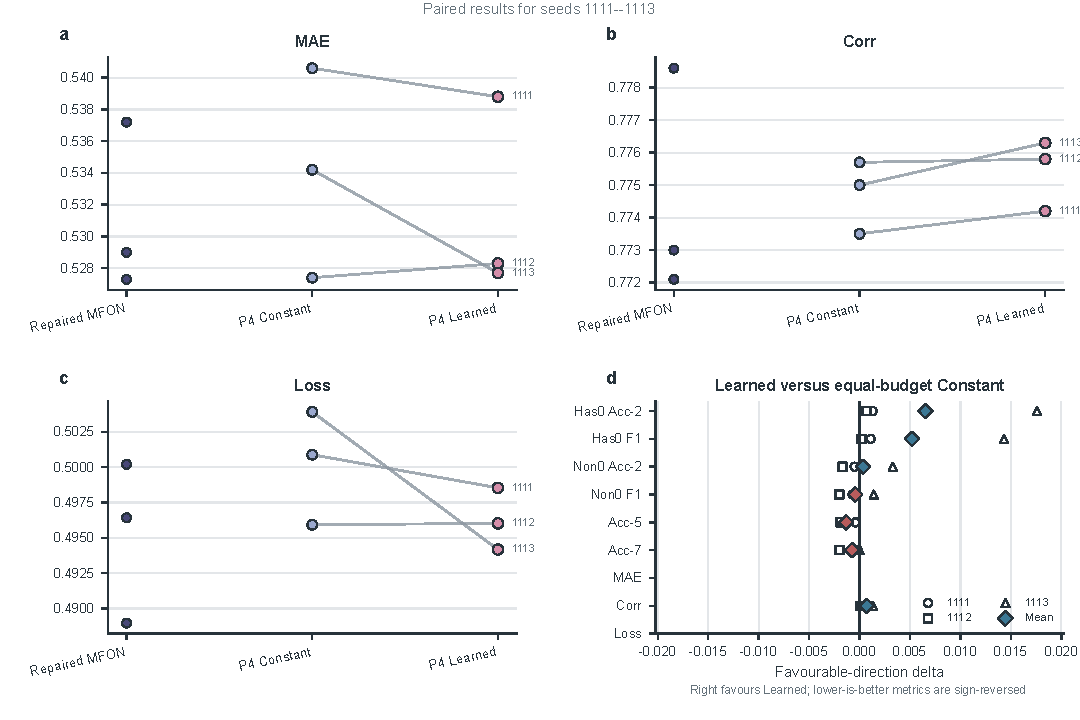
\includegraphics[width=\textwidth]{../figures/f2_mosei_main_results_en.pdf}
\caption{Paired frozen MOSEI task results under an equal auxiliary budget.
\textbf{a--c}, Per-seed MAE, correlation, and test loss for repaired MFON, P4
Constant, and P4 Learned. Lines connect Constant and Learned results obtained
with the same seed; repaired-MFON points are references and are not joined
because that comparison also changes the reliability-training path.
\textbf{d}, Per-seed favourable-direction differences between Learned and
Constant across all endpoints; diamonds show the three-seed mean, and MAE and
loss are sign-reversed so that right consistently favours Learned. The visible
heterogeneity and mixed classification effects are descriptive ($n=3$ seeds)
and do not constitute a significance test. Source data include every plotted
seed.}
\label{fig:mosei-main-results}
\end{figure*}

\subsection{Cross-corruption reliability stress
audit}\label{cross-corruption-audit}

To test whether the heads recognize only the Gaussian pattern used in
training, we audited all 4,659 MOSEI test samples for every frozen Learned
checkpoint. Gaussian audits use multiple severities. Timestep dropout and
contiguous masking use severity 0.75, temporal shift circularly moves active
steps by up to half the valid sequence, and modality missing zeros all active
features. Every transformation preserves padding.

\begin{table*}[t]
\caption{Gaussian reliability audit on frozen MOSEI P4 Learned checkpoints
(mean $\pm$ sample standard deviation over three seeds).}
\label{tab:mosei-gaussian-audit}
\centering
\resizebox{\textwidth}{!}{%
\begin{tabular}{lccc}
\toprule
Modality & Spearman $\downarrow$ & AUROC $\uparrow$ & Highest below clean $\uparrow$ \\
\midrule
Vision & $-0.931602\pm0.007408$ & $0.972161\pm0.009176$
& $0.985905\pm0.000328$ \\
Audio & $-0.830330\pm0.005901$ & $0.999982\pm0.000014$
& $1.000000\pm0.000000$ \\
\bottomrule
\end{tabular}%
}
\end{table*}

The Gaussian response is stable across seeds, but clean scores retain
correlations with simple statistics: visual length $0.1008\pm0.0400$, visual
energy $-0.1358\pm0.0791$, acoustic length $0.2194\pm0.0384$, and acoustic
energy $-0.2705\pm0.1630$. Correlations with absolute sentiment labels are
small (visual $0.0185\pm0.0200$; acoustic $0.0261\pm0.0115$), although these
checks cannot exclude other confounds.

\begin{figure*}[t]
\centering
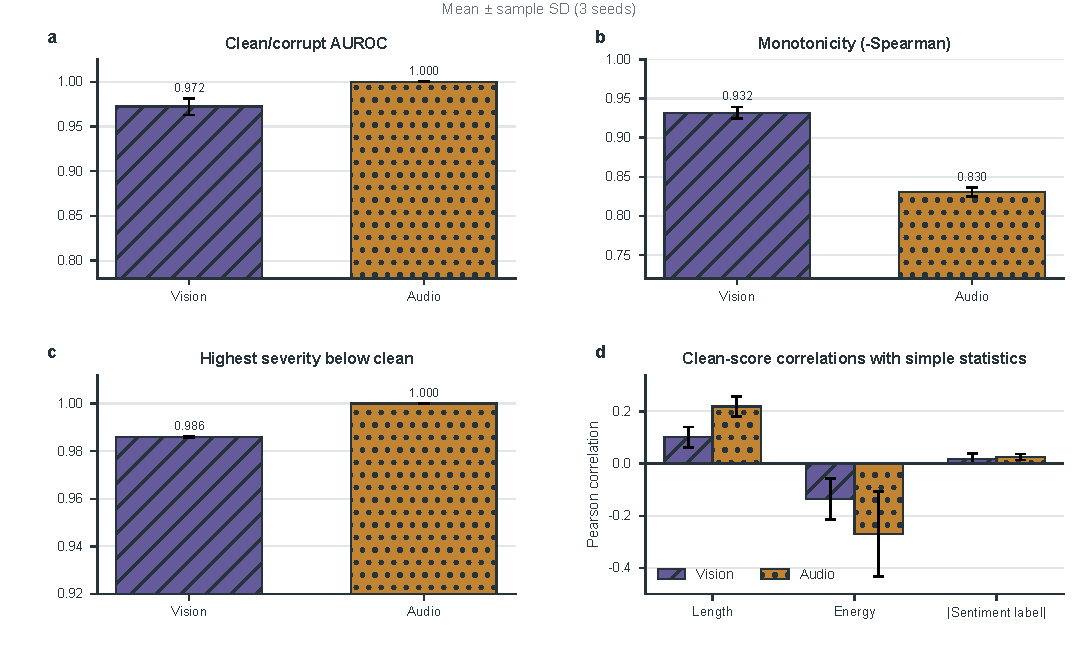
\includegraphics[width=\textwidth]{../figures/f3_mosei_gaussian_audit_en.pdf}
\caption{In-family Gaussian reliability and residual confound audit.
\textbf{a}, Clean/corrupt AUROC. \textbf{b}, Negative Spearman correlation
between corruption severity and reliability score, plotted so that larger
values indicate stronger monotonic decrease. \textbf{c}, Fraction of
highest-severity scores below the paired clean score. \textbf{d}, Pearson
correlations between clean reliability scores and feature length, feature
energy, or absolute sentiment label. Bars and error bars show mean $\pm$
sample standard deviation over the three frozen seeds; each seed audits all
4,659 MOSEI test samples. The heads detect the Gaussian corruption used in
training, while the correlations in panel d motivate a bounded rather than
universal reliability claim. Source data are provided with the figure files.}
\label{fig:mosei-gaussian-audit}
\end{figure*}

\begin{table*}[t]
\caption{MOSEI cross-corruption stress audit. AUROC measures clean/corrupt
separation; $\Delta$MAE is corrupt minus clean. Values are mean $\pm$ sample
standard deviation over three seeds.}
\label{tab:mosei-cross-corruption}
\centering
\small
\textbf{(a) Clean/corrupt detection AUROC}\par\smallskip
\begin{tabular*}{\textwidth}{@{\extracolsep{\fill}}lrr@{}}
\toprule
Corruption & Vision $\uparrow$ & Audio $\uparrow$ \\
\midrule
Timestep dropout (0.75) & $0.498965\pm0.003535$ & $0.593710\pm0.022123$
\\
Contiguous mask (0.75) & $0.541152\pm0.011892$ & $0.754388\pm0.009935$
\\
Temporal shift (1.00) & $0.509639\pm0.002927$ & $0.511274\pm0.002509$
\\
Modality missing (1.00) & $0.407169\pm0.227165$ & $0.999857\pm0.000248$
\\
\bottomrule
\end{tabular*}

\vspace{0.65em}
\textbf{(b) Task sensitivity: corrupt-minus-clean MAE}\par\smallskip
\begin{tabular*}{\textwidth}{@{\extracolsep{\fill}}lrr@{}}
\toprule
Corruption & Vision $\Delta$MAE & Audio $\Delta$MAE \\
\midrule
Timestep dropout (0.75) & $+0.000933\pm0.000153$ & $+0.000067\pm0.000058$ \\
Contiguous mask (0.75) & $+0.001700\pm0.000721$ & $+0.000067\pm0.000058$ \\
Temporal shift (1.00) & $-0.000133\pm0.000058$ & $0.000000\pm0.000000$ \\
Modality missing (1.00) & $+0.012700\pm0.003110$ & $+0.003600\pm0.003195$ \\
\bottomrule
\end{tabular*}
\end{table*}

\begin{figure*}[t]
\centering
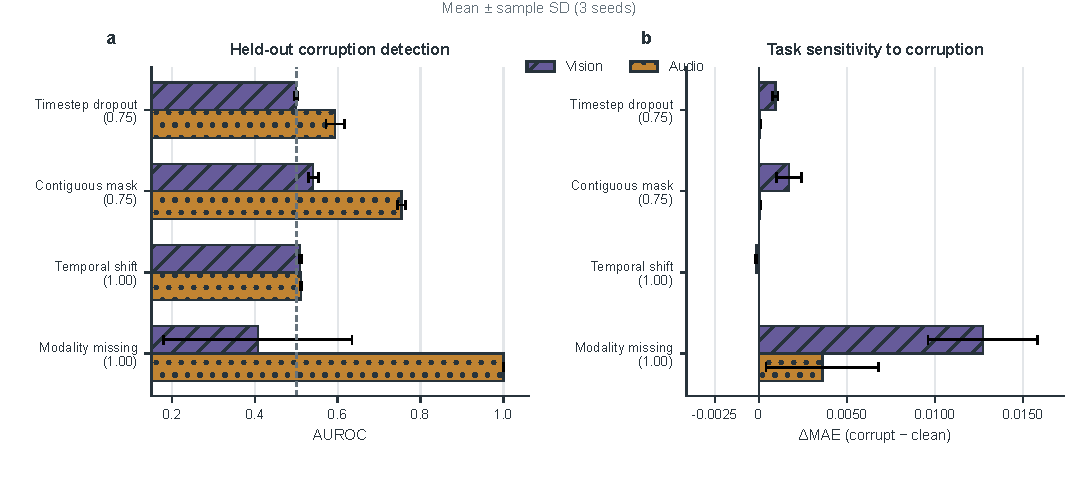
\includegraphics[width=\textwidth]{../figures/f4_mosei_cross_corruption_en.pdf}
\caption{Held-out corruption detection and task sensitivity. \textbf{a},
Clean/corrupt AUROC for visual and acoustic timestep dropout, contiguous
masking, temporal shift, and modality missing; the dashed line marks chance
AUROC of 0.5. \textbf{b}, Change in task MAE after the same corruption,
computed as corrupt minus clean. Bars and error bars show mean $\pm$ sample
standard deviation over three frozen seeds, with all 4,659 MOSEI test samples
audited per seed. Near-chance detection for several perturbations and the
mismatch between acoustic detectability and task effect show that degradation
detection is not equivalent to general reliability or task utility. Source
data are provided with the figure files.}
\label{fig:mosei-cross-corruption}
\end{figure*}

Three boundaries follow. First, Gaussian reliability is not a general quality
estimate: visual detection is near random for timestep dropout and temporal
shift, and acoustic detection is only moderate for contiguous masking.
Second, complete absence is asymmetric. Acoustic absence is almost perfectly
detected, whereas visual absence produces below-chance mean AUROC with large
seed variation. Third, degradation detectability is not task utility.
Acoustic interventions barely change predictions, while missing vision
increases MAE by 0.0127 on average. We therefore restrict the claim to
reliability under the Gaussian training intervention and fixed-budget
auxiliary allocation, rather than cross-corruption quality estimation or
missing-modality robustness.

\subsection{Cross-sample target-fidelity
audit}\label{cross-sample-target-fidelity-audit}

We performed a post-hoc exploratory audit on the MOSEI validation split of
each frozen Learned checkpoint ($n=1{,}871$ per seed). The primary proxy was
negative per-sample KL, whose definition is stable across mini-batches.
InfoNCE and the coefficient-weighted proxy
$0.3\,\mathrm{KL}+0.001\,\mathrm{InfoNCE}$ were compared only within their
generating mini-batches because their negative sets vary across batches.

Visual scores consistently contradicted the proposed fidelity direction.
Across seeds, global Spearman correlation with negative KL was
$-0.315423\pm0.069633$, partial Spearman after controlling active length and
feature energy was $-0.248627\pm0.064859$, and pairwise concordance was
$0.393666\pm0.023143$. Acoustic associations were weak:
$0.092174\pm0.042066$, $0.072239\pm0.067445$, and
$0.529795\pm0.014286$, respectively. Within-batch weighted-proxy Spearman was
$-0.290099\pm0.047795$ for vision and $0.064885\pm0.047447$ for audio. Thus,
Gaussian degradation ordering does not establish that higher clean-sample
scores identify more trustworthy auxiliary targets. We retain this negative
result and do not reinterpret the score direction after observing it.

\subsection{Efficiency and resource cost}\label{efficiency-audit}

We ran a uniform microbenchmark on one NVIDIA GeForce RTX 4090 D using the
same 32-sample MOSEI test batch and frozen seed-1111 checkpoint for every
variant. Each method used three warmup iterations and 20 timed repetitions.
Inference covers the end-to-end forward pass; the training measurement covers
forward and backward computation but excludes data loading, the optimizer
update, and checkpoint writing. Latency is therefore a within-session mean,
not a cross-device or cross-seed statistic.

\begin{table*}[t]
\caption{Single-batch MOSEI efficiency audit under identical hardware,
inputs, and timing protocol. Reliability branches execute only during P4
training.}
\label{tab:efficiency-audit}
\centering
\small
\textbf{(a) Model size and peak allocated memory}\par\smallskip
\resizebox{\textwidth}{!}{%
\begin{tabular}{lrrrrr}
\toprule
Method & Opt. params (M) & Added rel. params & Ckpt. (MiB)
& Inf. peak (GiB) $\downarrow$ & F+B peak (GiB) $\downarrow$ \\
\midrule
Repaired MFON & 130.765 & 0 & 585.14 & 1.136 & 4.791 \\
P4 Constant & 130.796 & 30,914 & 585.14 & 1.136 & 4.805 \\
P4 Learned & 130.796 & 30,914 & 585.14 & 1.136 & 4.805 \\
\bottomrule
\end{tabular}%
}

\vspace{0.7em}
\textbf{(b) Runtime}\par\smallskip
\begin{tabular}{lrrr}
\toprule
Method & Inf. (ms/batch) $\downarrow$ & Samples/s $\uparrow$
& F+B (ms/batch) $\downarrow$ \\
\midrule
Repaired MFON & 1040.20 & 30.76 & 1112.09 \\
P4 Constant & 1009.84 & 31.69 & 1135.09 \\
P4 Learned & 1024.97 & 31.22 & 1120.03 \\
\bottomrule
\end{tabular}
\end{table*}

P4 adds 30,914 optimized reliability parameters, approximately 0.024\% of
the repaired-MFON optimizer parameter count. All variants instantiate the
same model class, so stored parameters (153.347M) and checkpoint size are
identical; reliability branches are inactive at inference, and inference peak
memory is also identical. Relative to repaired MFON, Learned shows 1.46\%
lower observed inference latency, 0.71\% higher forward-plus-backward latency,
and 0.29\% higher peak training memory. Because these small timing differences
come from one sequential session, we do not interpret them as speedups. The
supported conclusion is small additional parameter and training-memory cost
without an expanded deployed inference graph.

\begin{figure*}[t]
\centering
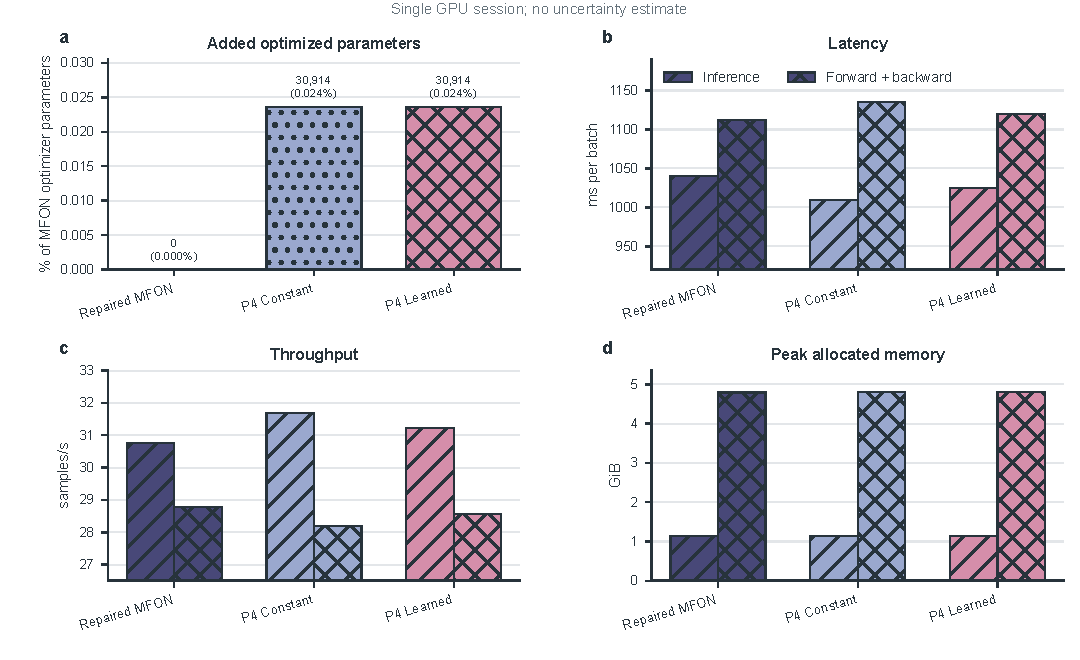
\includegraphics[width=\textwidth]{../figures/f5_mosei_efficiency_en.pdf}
\caption{Single-GPU parameter, runtime, and memory audit. \textbf{a}, Added
optimized reliability parameters as a percentage of the repaired-MFON
optimizer scope. \textbf{b--d}, Inference and forward-plus-backward latency,
throughput, and peak allocated memory. All variants use the same seed-1111
checkpoint protocol, one 32-sample MOSEI batch, one NVIDIA GeForce RTX 4090 D,
three warmup iterations, and 20 timed repetitions. The measurements are
single-session means without uncertainty estimates; data loading, optimizer
updates, and checkpoint writes are excluded from forward-plus-backward timing.
All checkpoints are 585.14 MiB, and the reliability branch is absent from
deployed inference. Source data are provided with the figure files.}
\label{fig:mosei-efficiency}
\end{figure*}

\FloatBarrier

\section{Discussion}\label{discussion}

\subsection{What the current evidence
establishes}\label{what-the-current-evidence-establishes}

The strongest conclusion is methodological rather than
leaderboard-oriented. A quality-aware mechanism should not be trusted
merely because it contains a scalar named quality. The norm-proxy audit
demonstrates how a plausible score can reverse the intended degradation
ordering, and the implementation audit demonstrates how nominally
sample-wise weighting can disappear through batch reduction. The final
P4 design removes these two ambiguities: reliability remains a sample
vector, losses remain unreduced until weighting, and every batch
preserves the same mean auxiliary budget.

Under these controls, P4 Learned improves mean MAE, correlation, and test loss
over P4 Constant on both the exploratory MOSI study and the frozen-protocol
MOSEI replication. This is consistent with a small mean allocation effect
under a fixed budget, but does not establish stability. MOSEI fine-grained
metrics and Non0 F1
do not improve simultaneously, however, and Learned does not improve MAE or
loss over repaired MFON. The replication therefore supports a descriptive
primary-endpoint mean direction against the equal-budget Constant control, not
uniform performance gains. Three seeds remain descriptive and are
insufficient for statistical-significance claims.

The comparison with Constant does not by itself justify the direction of
allocation. In the final-schedule seed-1111 comparison,
Learned was better than Permuted and Inverse on MAE, but Inverse was better by
0.0001 on correlation. These small contrasts neither establish a stable
score--sample correspondence effect nor validate positive allocation. The
defensible claim remains a descriptive task difference under a fixed budget,
not that higher-reliability weighting is universally optimal.

The cross-sample validation audit gives a sharper mechanism boundary. Visual
reliability scores are consistently anti-aligned with KL target fidelity, and
acoustic scores show only weak alignment. The favorable Learned-versus-Constant
task means therefore cannot be attributed to the stated assumption that higher
scores identify cleaner auxiliary targets. The seed-1111 Permuted and Inverse
controls add a limited task comparison, while cross-seed replication and
component attribution remain open.

\subsection{Why reliability measurement does not imply robust
fusion}\label{why-reliability-measurement-does-not-imply-robust-fusion}

The reliability heads achieve high AUROC under the Gaussian training
corruption, yet AUROC approaches 0.5 under unseen timestep dropout and
temporal shift. Isolated acoustic interventions also barely change sentiment
predictions, whereas complete visual absence causes a clearer MAE increase.
Thus, corruption detectability and task utility are distinct. A likely
explanation is text dominance in the MFON checkpoints: auxiliary reliability
can shape representation learning without causing a large inference-time
change in the final prediction. Accordingly, the method is
\emph{reliability-aware auxiliary-supervision allocation}, not a demonstrated
inference-time robust fusion mechanism.

\subsection{Alternative explanations and open
confounds}\label{alternative-explanations-and-open-confounds}

The acoustic reliability score retains a recurring correlation with
effective length. This could reflect a residual shortcut, a genuine relation
between temporal evidence and corruption detectability, or both.
Padding-preserving and cross-corruption audits on MOSEI do not resolve the
alternatives. The acoustic head detects all-zero absence and Gaussian noise
reliably, detects contiguous masking only moderately, and barely detects
temporal shifts; the visual head is unstable under all-zero absence. These
scores should therefore be interpreted as responses to the training
corruption family, not as general perceptual-quality estimates.

Feature-level synthetic corruptions provide ordered and controlled
interventions, but they are not equivalent to automatic-speech-recognition
errors, real background mixtures, natural facial occlusion, or upstream
feature-extraction failures. The added timestep-dropout, contiguous-mask,
temporal-shift, and modality-missing audits broaden the stress envelope while
directly exposing poor cross-corruption transfer. Deployment-related claims
would still require corruptions of the original audio and video streams.

\subsection{Relation to existing quality-aware
methods}\label{relation-to-existing-quality-aware-methods}

The contribution is not the generic idea of reliability weighting,
corruption ranking, or maintaining an expected weight. These ideas have
close precedents in dynamic fusion and supervised low-quality learning
\cite{zhang2023qmf, mai2025samlml}. The narrower contribution is an
audit-and-control package for training-time auxiliary learning: test the
score, retain loss granularity, hold the finite-batch budget exactly
constant, and compare sample assignments without changing total
supervision. Whether this package transfers beyond MFON remains an
empirical question rather than an established model-agnostic property.

\section{Limitations, Reproducibility, and Responsible
Use}\label{limitations-reproducibility-and-responsible-use}

This study has six primary empirical limitations. First, MOSI test-split
reliability diagnostics informed visual-head retention and acoustic-head
redesign, so MOSI remains exploratory rather than untouched validation.
Second, although the frozen three-seed MOSEI replication is complete, three
seeds do not support statistical significance and primary endpoints do not
uniformly improve over repaired MFON. Third, the post-hoc MOSEI validation
audit contradicts cross-sample KL fidelity for vision and provides only weak
acoustic support; inverse/difficulty-aware and permutation controls are
complete only for seed 1111. Fourth, interventions operate on pre-extracted
features, and the new non-Gaussian audits reveal substantial cross-corruption
failure rather than replacing real-media noise, occlusion, and misalignment
experiments. Fifth, evidence covers only MFON and does not establish model
independence or missing-modality robustness. Sixth, MOSI repaired-MFON test
loss is unavailable; the efficiency audit also covers only one GPU, one batch
shape, and a microbenchmark without data loading or optimizer updates, so it
does not establish cross-hardware or full-training-cycle cost.

Reproducibility controls include fixed seeds, validation-based
checkpoint selection, unit tests for mathematical contracts, explicit
logging of score and weight means and standard deviations, and a staged
cross-dataset gate. The repository should release code and lightweight
configuration files but does not redistribute dataset files, BERT
weights, private checkpoints, credentials, or personal attachments.

Sentiment prediction should not be interpreted as a direct measurement
of a person's psychological state, intent, political position, or
truthfulness. Any later deployment should use uncertain or
low-reliability outputs as a prompt for human review rather than as an
autonomous basis for sanctions, profiling, or other high-impact
decisions.

\section{Conclusion}\label{conclusion}

This study reframes quality-aware multimodal sentiment analysis as an
auditable optimization problem. We identify failures caused by
batch-level score aggregation, premature loss reduction, unconstrained
auxiliary weights, and a norm proxy that rewards stronger corruption. We
then learn modality reliability from ordered Gaussian interventions and use it to
redistribute per-sample MFON auxiliary losses under an exact
finite-batch budget. Exploratory three-seed MOSI results motivate learned
redistribution for binary and regression-oriented metrics, while fine-grained
classification remains mixed. Exploratory MOSI and frozen MOSEI three-seed
results both favor Learned over equal-budget Constant on mean MAE,
correlation, and test loss, but repaired MFON is not uniformly surpassed.
Cross-corruption audits show limited transfer, while the cross-sample
validation audit finds visual anti-alignment and only weak acoustic alignment
with KL target fidelity. A uniform microbenchmark finds that P4 adds approximately
0.024\% optimized parameters; Learned increases forward-plus-backward latency
and peak training memory by 0.71\% and 0.29\% relative to MFON without
expanding the deployed inference graph. Acoustic length dependence,
text-dominant inference, failed cross-sample target fidelity, incomplete
final-schedule actionability controls, and the lack of real-media stress tests
bound the scope. The evidence establishes a transparent and falsifiable
audit-and-budget-control mechanism, not a general quality estimator, a
validated allocation direction, or a robust-fusion model.
